\begin{tabular}{l l}
        \multirow{3}{*}{
\includegraphics[width=1.5cm]{Imagenes/imanol.jpg}} &  \\
        & \textbf{Rivero Ronquillo Omar Imanol}\\
        & \\
    \end{tabular}
    \vspace*{3\baselineskip}\\
    Nunca había pensado en las formas en las que se podría optimizar la solución a un problema por medio de un algoritmo programable. Me pareció un enfoque increíble y ahora me parece que tengo claro porque se usan estos algorimos y en qué problemas se les podría dar un uso. A pesar de que en comparación con las prácticas anteriores se tuvieron que incluir más cosas además de los algorimos, para poder probarlos y estudiarlos, me parecieron un gran complemento en mi formación académica.
    
    En conclusión, me gustaría conocer más algoritmos de este tipo, me interesaron especialmente los algoritmos de compresión, aunque puedo estar bastante seguro de que las compresiones modernas deberán de tener una complejidad mayor de aprenderse y comprender su funcionamiento, que seguramente justificaran todo esto con las tasas de compresiones que puedan lograr.
    \\\\
    \begin{tabular}{l l}
        \multirow{3}{*}{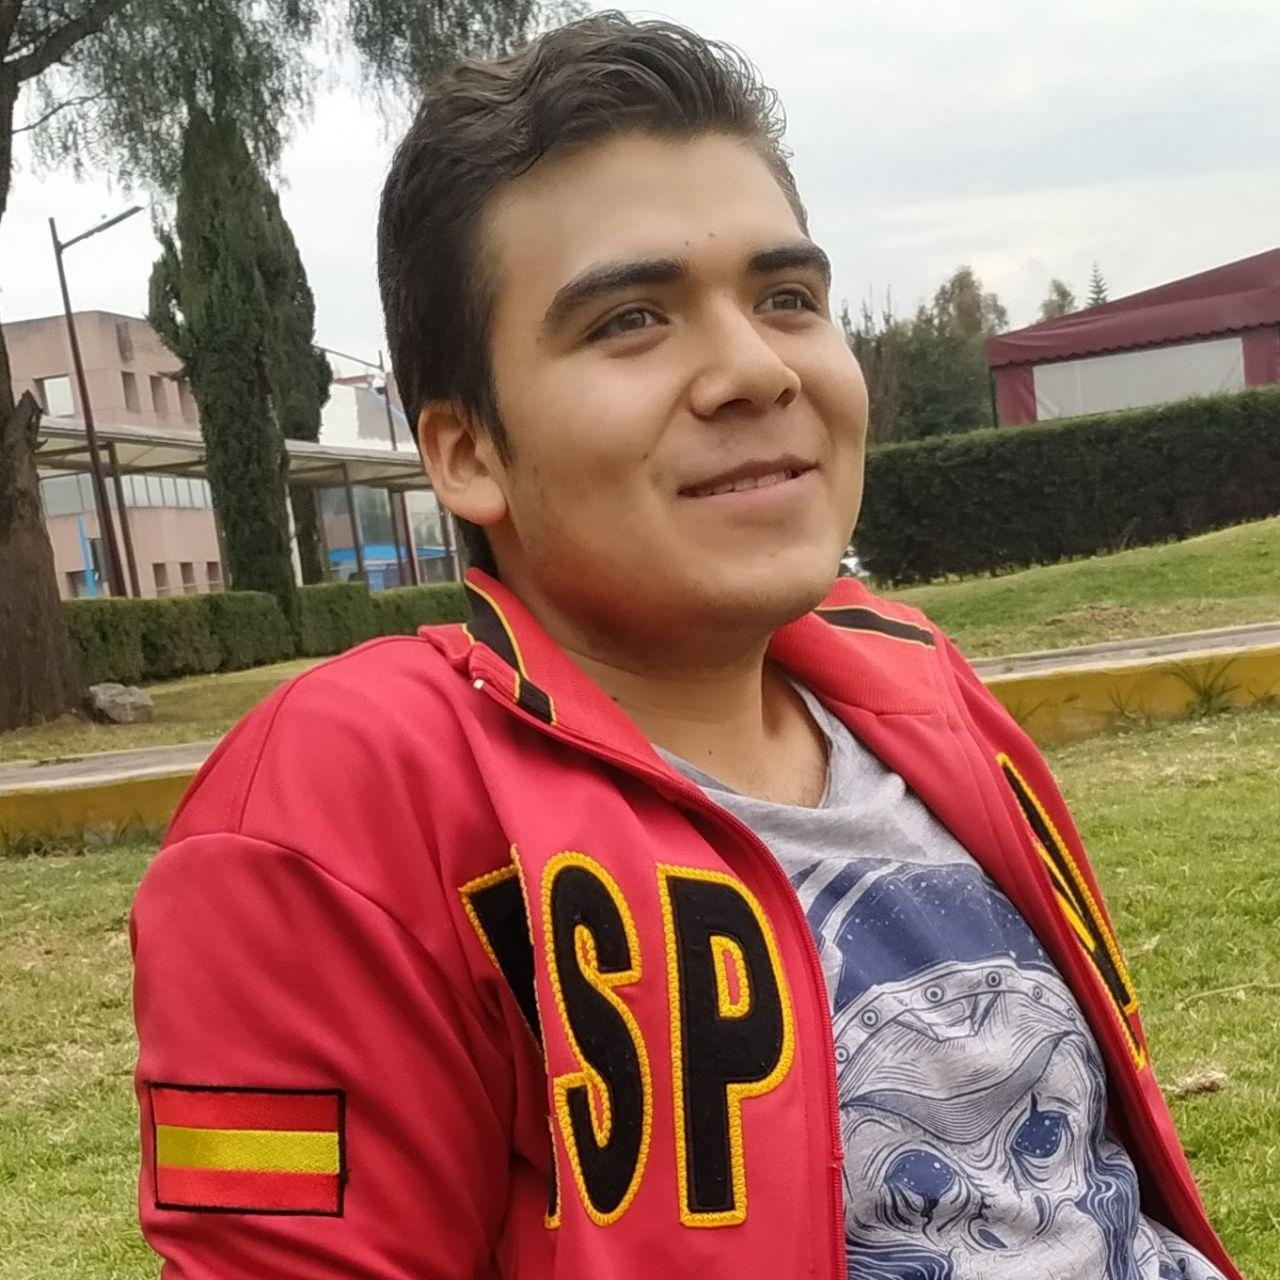
\includegraphics[width=1.5cm]{Imagenes/lalo.jpg}}  &  \\
        & \textbf{Valle Mart\'inez Luis Eduardo} \\
        & \\
    \end{tabular}
    \vspace*{3\baselineskip}\\
    